\section{The Interface}
Next, we will describe the components of the \sys interface used in this demonstration.


\begin{figure}[t]
\centering
 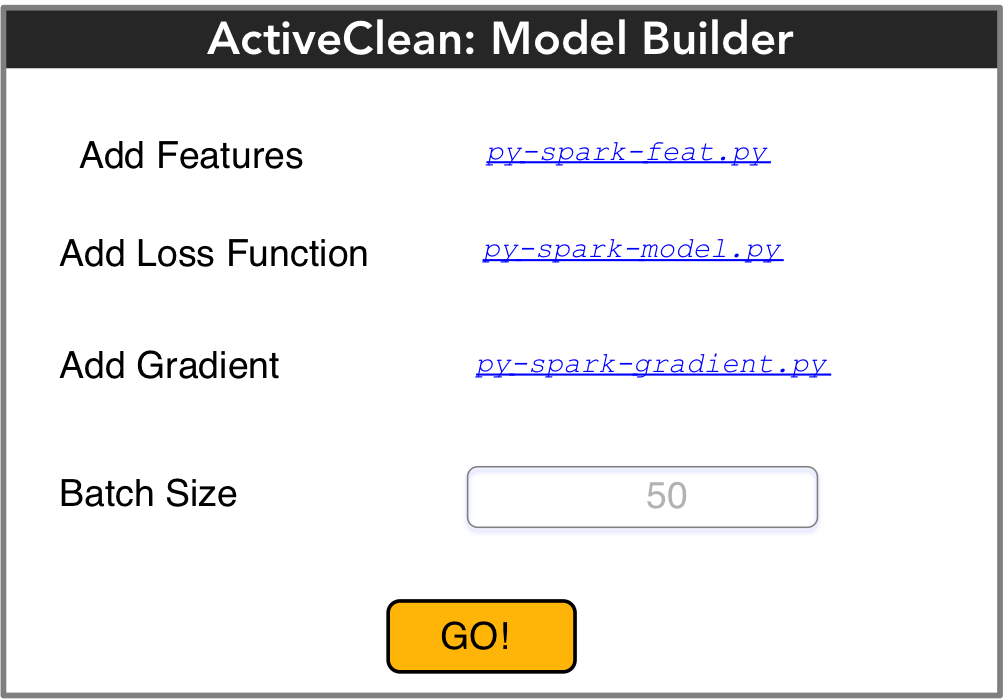
\includegraphics[width=0.48\columnwidth]{figs/interface1.png}
 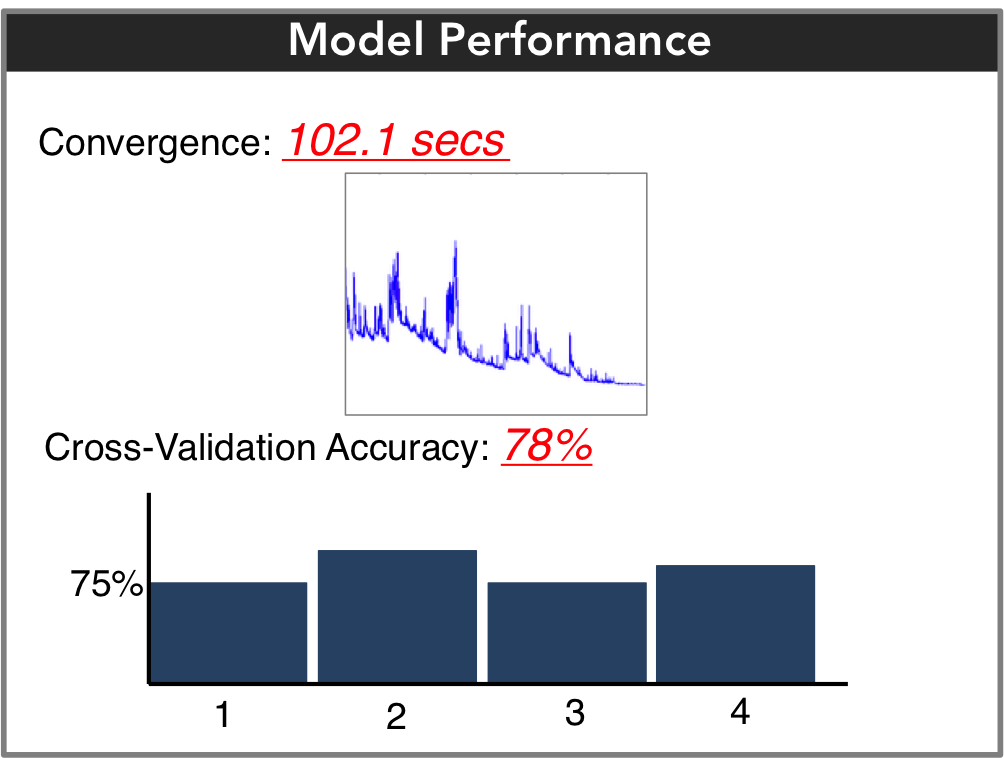
\includegraphics[width=0.48\columnwidth]{figs/interface2.png}
 \caption{Initial Run. The analyst loads user-defined model functions into \sys and then trains an initial model on the dirty data \label{irun}}
\end{figure}

\subsection{The Intial Run}
The first part of \sys is called the \textsf{Model Builder}, this is an interface that the analyst uses to specify the problem.
She loads three user-defined functions written in PySpark~\cite{pyspark} based on the descriptions in the previous section.
Optionally, she can change the batch size from our default setting of 50.
Once the model is instantiated, then she can train the model on the dirty data.
If there are any errors that are critical, i.e., causes the training to fail, \sys will immediately error.
However, if the training proceeds to completion, the analyst will see the \textsf{Performance} window which plots the model's convergence as a function of iteration.
It also shows the cross-validation accuracy if it is a classification task and the hold-out residual error if it is a regression task.
Both of these panels are visualized in Figure \ref{irun}.

\subsection{Diagnose Interface}
Suppose the analyst is unhappy with her model, and wishes to understand why her prediction accuracy is poor.
She can then open the diagnose panel to understand why (Figure \ref{diag}).
When she opens the diagnose panel, \sys applies the importance sampling algorithm to select a subset of examples from the dataset.
Since these points are in general high dimensional, we apply T-SNE~\cite{van2008visualizing} to visualize the points in 2D.
T-SNE is a non-linear dimensionality reduction technique which is widely used to visualize complex data distributions.
In the diagnose interface, we use color coding to indicate class in the case of classification.
The analyst can select examples from the diagnose interface for further inspection.

\begin{figure}[t]
\centering
 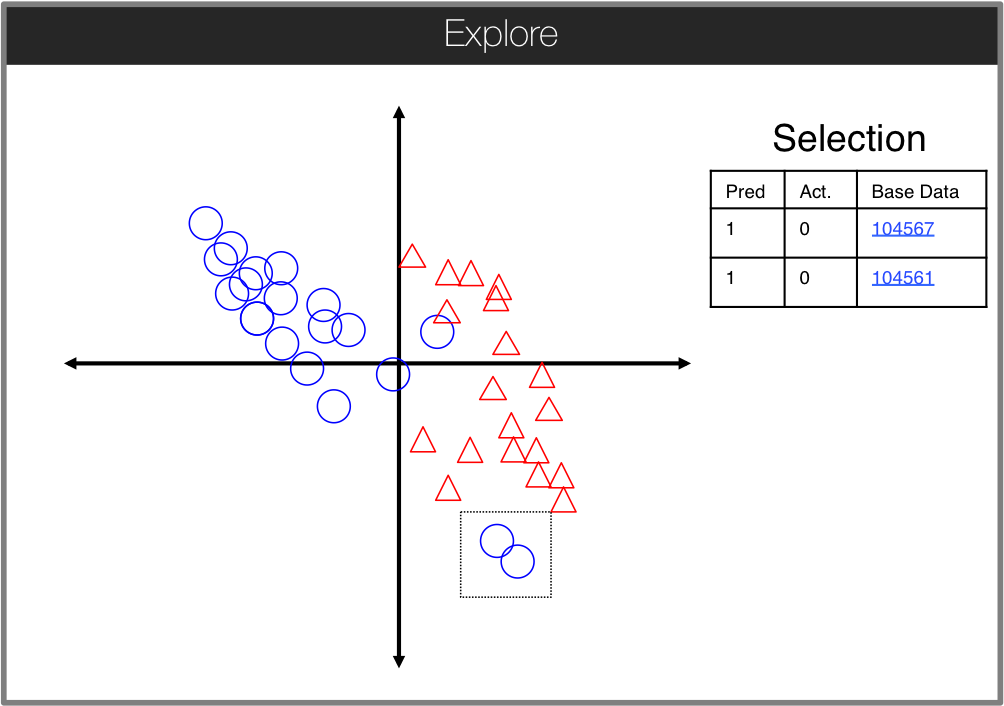
\includegraphics[width=0.6\columnwidth]{figs/interface3.png}
 \caption{The diagnose inteface. The analyst can select and inspect suspect data. \label{diag}}
\end{figure}

\subsection{Clean Interface}

\begin{figure}[t]
\centering
 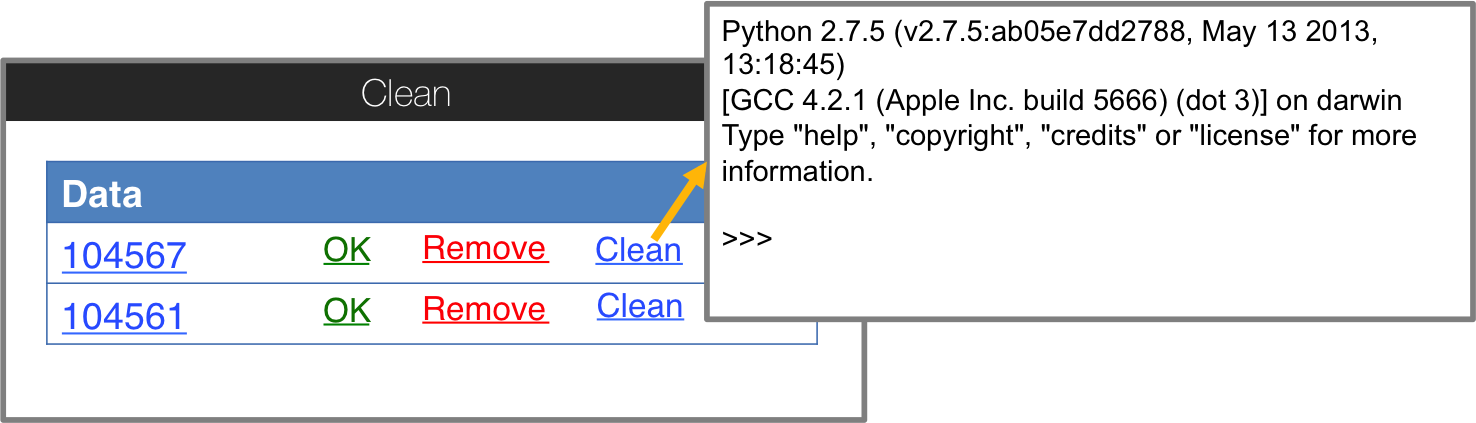
\includegraphics[width=\columnwidth]{figs/interface4.png}
 \caption{Clean Eval}
\end{figure}

\subsection{Iteration and Updates}

\begin{figure}[t]
\centering
 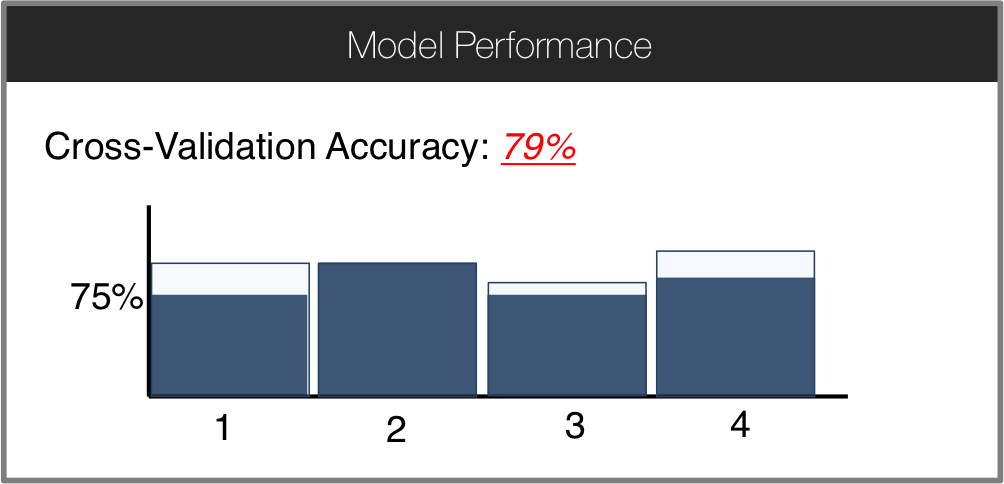
\includegraphics[width=0.6\columnwidth]{figs/interface5.png}
 \caption{Clean Eval}
\end{figure}